% !TEX program = xelatex


% Joint Programme with University of Information Technology, VNU-HCM
% Module: Individual Honours Project
%
% -----
%
% A Game-Based Approach to Motor Imagery Adaptation and BCI Calibration
% Author: Cao Đăng Khoa (dang.cao@mail.bcu.ac.uk)
% Student ID: 25195675
%
% Supervisor: Dr. Vi Chí Thành (vcthanh@hcmiu.edu.vn)
%------------------------------------%



%------ DOCUMENT CONFIGURATION ------%
\documentclass[a4paper, 11pt, openany]{report}
\usepackage{layout}
\usepackage{fonts}
\usepackage{headerfooter}
\usepackage{frontmatter}
\usepackage{contents}
\usepackage{atbegshi}
\usepackage{graphicx}
\usepackage{booktabs}
\usepackage{array}
\usepackage{hyperref}
\usepackage{chngcntr}
\usepackage{float}
\counterwithout{figure}{chapter}
\counterwithout{table}{chapter}



\makeatletter
\let\ps@plain\ps@fancy
\makeatother


%------------------------------------%



%----------- FRONT MATTER -----------%
\begin{document}

% Title Page
\reportTitlePage
    {Project Final Progress Review}
    {BCG: A Game-Based Approach to Motor Imagery Adaptation and BCI Calibration}
    {Cao Đăng Khoa}{25195675}
    {Bachelor of Science with Honours Computer Science}
    {Dr. Vi Chí Thành}{January 12, 2026 to April 6, 2026}
    \thispagestyle{titlepage}

% Page numbering
\pagenumbering{roman}
\setcounter{page}{0}

% Table of Contents
\reportTableOfContents

% List of Figures
\reportListOfFigures

\reportListOfTables

%------------------------------------%

\cleardoublepage
\pagenumbering{arabic}

\setstretch{1.2} 
\setlength{\parskip}{8pt plus 2pt minus 1pt}


%------- INTERIM PROGRESS REVIEW -------%
\chapter{Progress to Date - Summary}    
    The project is now in the model training and game design phase, having successfully completed all foundational 
    infrastructure work since the Interim Progress Review in January 2026.  
    First, four EEG devices were investigated and compared, leading to the selection of the Emotiv EPOC X as the 
    primary experimental platform. The device is now fully configured, with a Python pipeline successfully streaming 
    real-time raw EEG data via the Cortex API. 
    Second, I used the MIMED public dataset to train two classification pipelines (CSP+LDA and CSP+SVM).
    Third, two game concepts were initally defined for the gamified calibration interface. 
    And finally, our abstract on the BCG approach was accepted at the BME 11 
    conference. The most significant finding to date is that 
    cross-subject classification accuracy on MIMED ranges from 42\% to 52\%, below the threshold required for reliable 
    BCI control. While MIMED is the most hardware-compatible dataset available, having been collected on the same Emotiv 
    EPOC X device, its limited trial pool of 240 samples is insufficient for CSP to generalise across subjects. This has 
    prompted a strategic review of the training approach, with larger benchmark datasets and pretrained deep learning models 
    currently being implemented.

\chapter{Artefact Design and Development}
    \section{Implementation and Current State}
        The BCG system is built around a core insight: if a game's objectives naturally require motor imagination, every in-game action becomes a labelled calibration trial without explicit prompting. The system has three components.

        \textbf{EEG Data Acquisition.} The Emotiv EPOC X was selected following a hands-on comparison of four consumer EEG devices. Its 14-channel layout reliably covers the C3/C4 motor cortex positions critical for Motor Imagery classification. Following a direct discussion with the Emotiv support team, Emotiv sponsored a six-month research licence granting access to raw EEG data via the Cortex API. A custom Python pipeline now streams this data in real time.
        \begin{figure}[H]
            \centering
            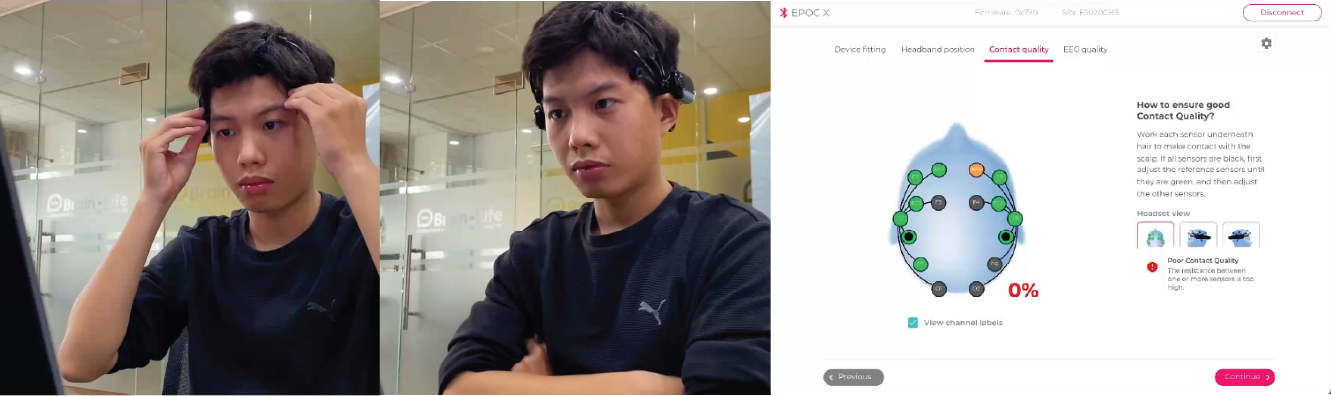
\includegraphics[width=1\textwidth]{Images/epocx_wearing.png}
            \caption{Author wearing the Emotiv EPOC X during device testing}
            \label{fig:epocx_wearing}
        \end{figure}
        \begin{figure}[h]
            \centering
            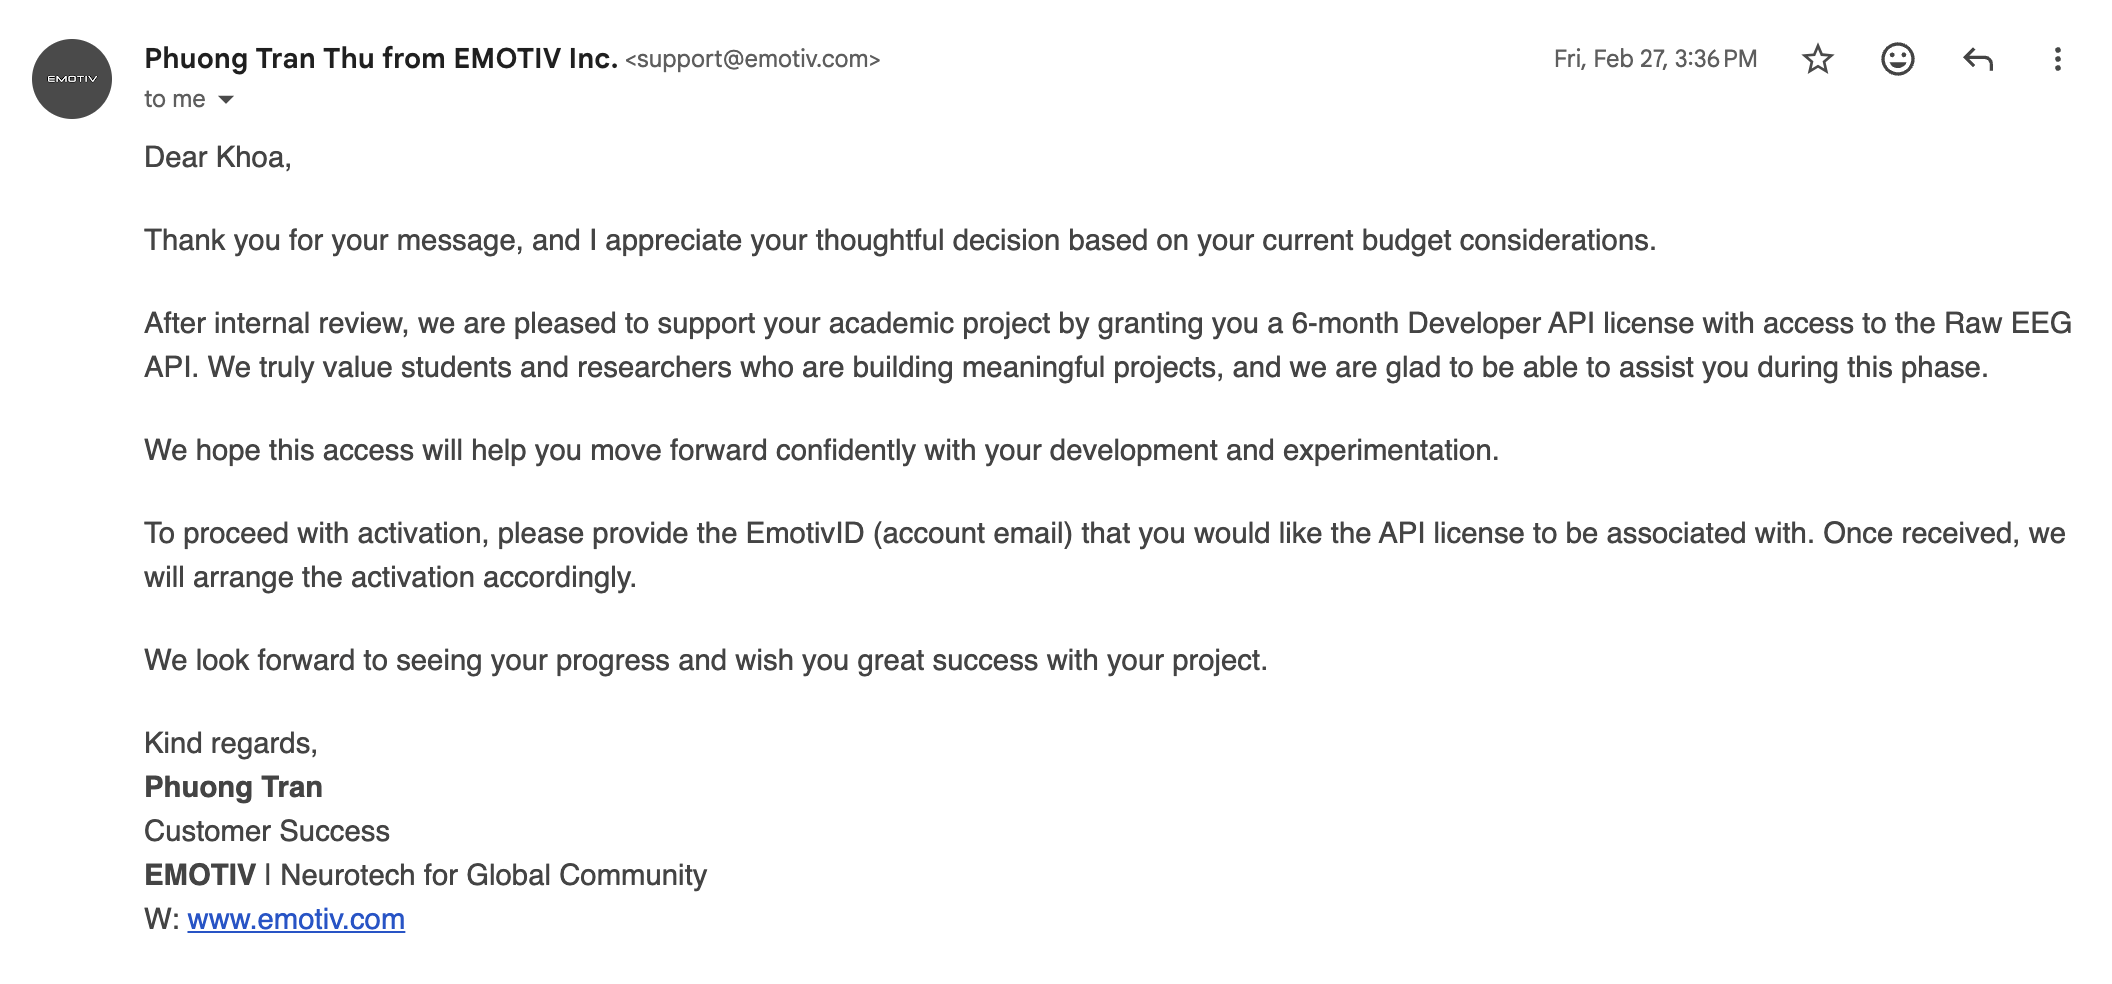
\includegraphics[width=1\textwidth]{Images/emotiv_support.png}
            \caption{Emotiv Developer API license approval email}
            \label{fig:emotiv_support}
        \end{figure}
        \vspace{1cm}

        \textbf{Signal Processing and Classification.} The initial pipeline bandpass filters raw EEG to 8-30 Hz, applies CSP for feature extraction, and classifies using LDA or SVM. MIMED was selected as the initial training dataset as it was recorded on the same Emotiv EPOC X device, minimising the domain gap. Benchmarked results are shown in Table 1.
        \newpage
        \begin{table}[h]
            \renewcommand{\arraystretch}{1.3}
            \centering
            \small
            \begin{tabular}{llll}
            \hline
            \textbf{Model} & \textbf{Dataset} & \textbf{Evaluation} & \textbf{Accuracy} \\
            \hline
            CSP + LDA & MIMED & Cross-subject, 5-fold & 52.5\% \\
            CSP + SVM & MIMED & Cross-subject, 5-fold & 46.7\% \\
            CSP + LDA & MIMED & Within-subject        & 42.1\% \\
            \hline
            \end{tabular}
            \caption{Initial classification results on the MIMED dataset}
            \label{tab:mimed_results}
        \end{table}

        The results, however, fall below the 70\% BCI control threshold due to MIMED's limited scale of 240 trials. Retraining on PhysioNet EEGMMIDB or fine-tuning EEGNetv4 are currently being evaluated.


        \textbf{Game Interface.} The game interface is being developed in GameMaker Studio 2, expected to be connected to the Python pipeline via a custom Cortex API bridge. The game is designed to make gameplay naturally drive motor imagination, with labelled calibration data collected implicitly in the background.

    \section{Analysis and Reflection}
       The key realisation from this phase is that BCG's value lies not in building a better classifier, 
       but in investigating whether natural, game-driven motor imagination can replace the repetitive cue-based 
       calibration protocol. This reframes the design priority: the game must feel spontaneous enough that the 
       player's MI signals are clean and consistent. Forced or distracted imagination produces weaker ERD/ERS 
       patterns; motivated, relaxed gameplay produces better data. This is why the game design is deliberately 
       simple, complexity would compete for the same cognitive bandwidth the BCI system needs to read.

        The MIMED results (42-52\%) reflect a cross-subject baseline on a small dataset, not the 
        final performance target. In the full system, the classifier will be updated continuously using 
        labelled data collected during gameplay, adapting to each user over time. The low initial accuracy 
        is expected, and the implicit collection mechanism is precisely how it will be addressed

\chapter{Updated Planning for Project Completion}
    \section{High-priority Tasks}
    
    The following high-priority tasks remain to complete the project:
    \begin{itemize}
        \item Finalise the classification pipeline by evaluating PhysioNet EEGMMIDB and EEGNetv4 as training alternatives
        \item Complete the BCG game prototype in GameMaker Studio 2 with left/right MI-driven controls
        \item Build and test the real-time Python-GameMaker communication bridge via the Cortex API
        \item Design the traditional baseline calibration protocol for the comparative user study
        \item Conduct a within-subjects user study with 8-10 participants, measuring classification accuracy and NASA-TLX workload
        \item Write and finalise the full dissertation
        \item Prepare the project poster and viva demonstration
    \end{itemize}

    \vspace{2cm}

    \begin{figure}[H]
        \centering
        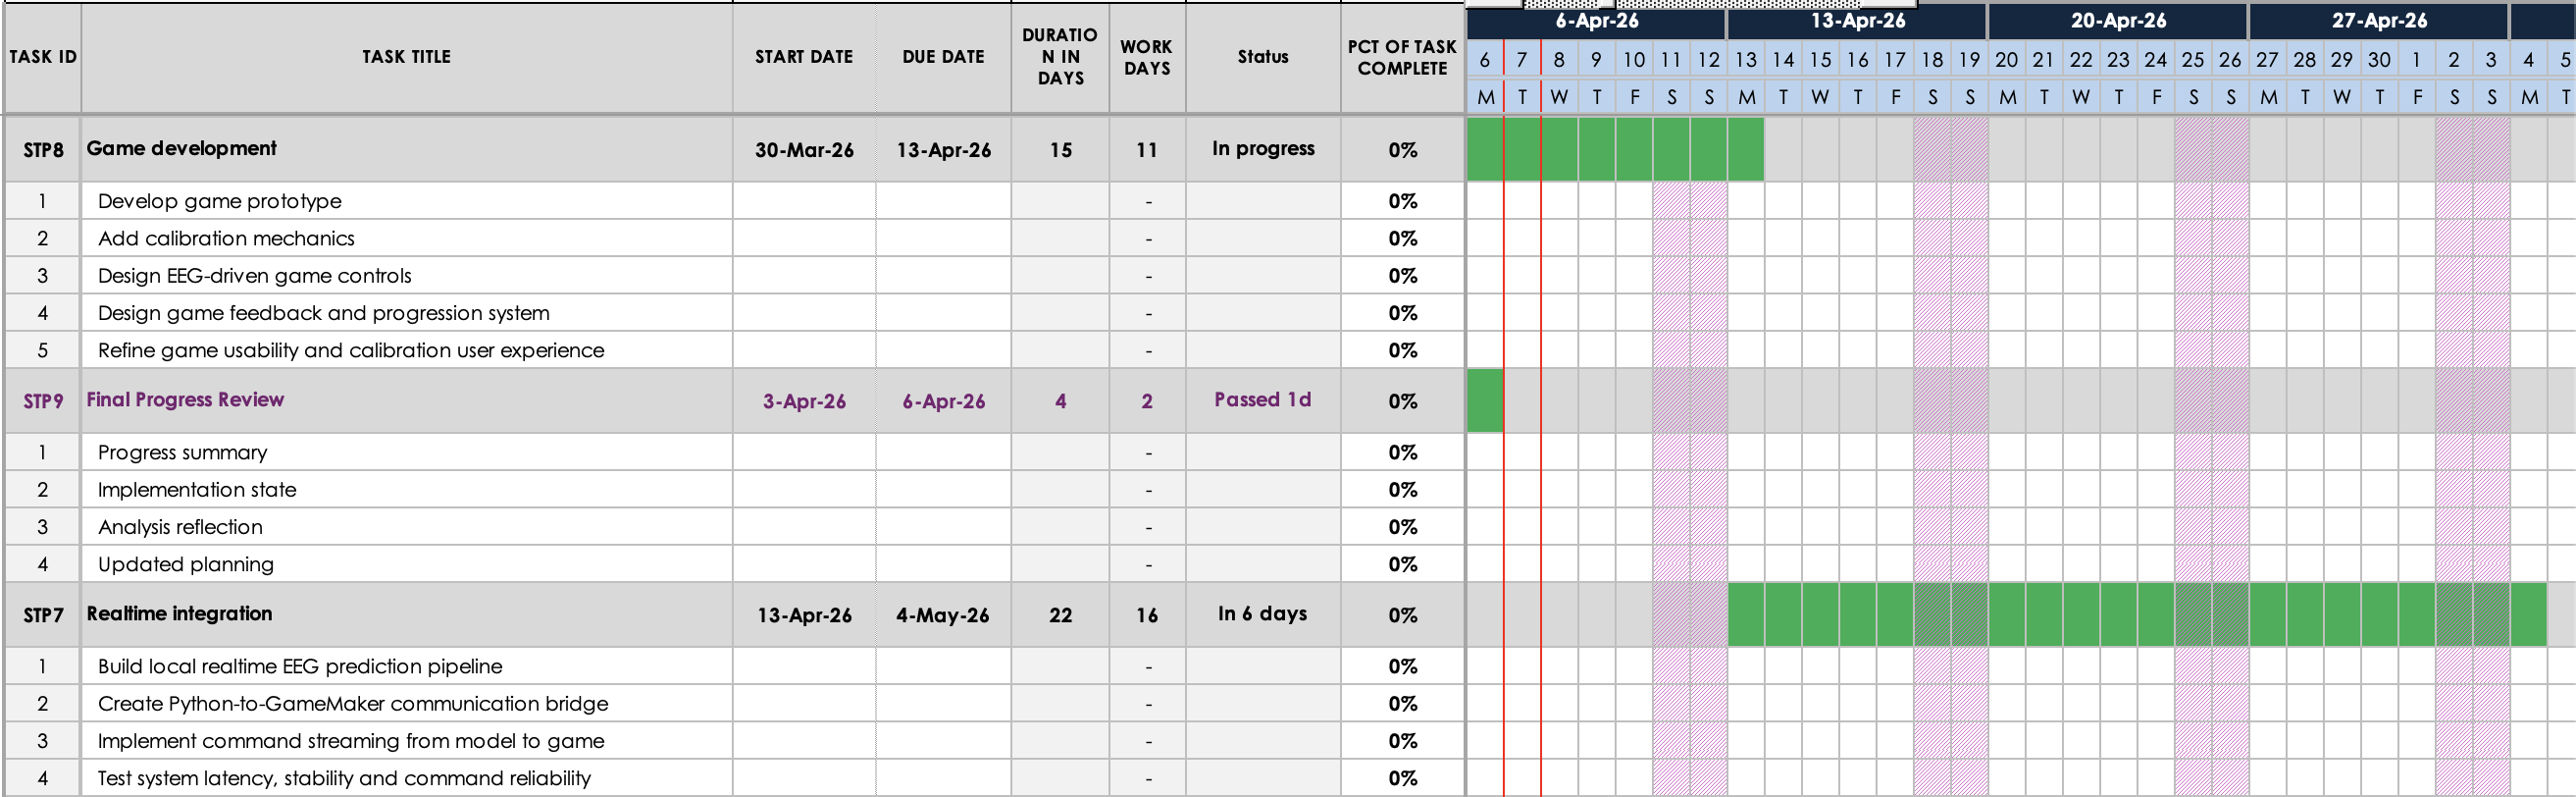
\includegraphics[width=1\textwidth]{Images/timeline-1.png}

        \caption{Project Timeline - April}
        \label{fig:timeline-1}
    \end{figure}
    
   \begin{figure}[H]
        \centering
        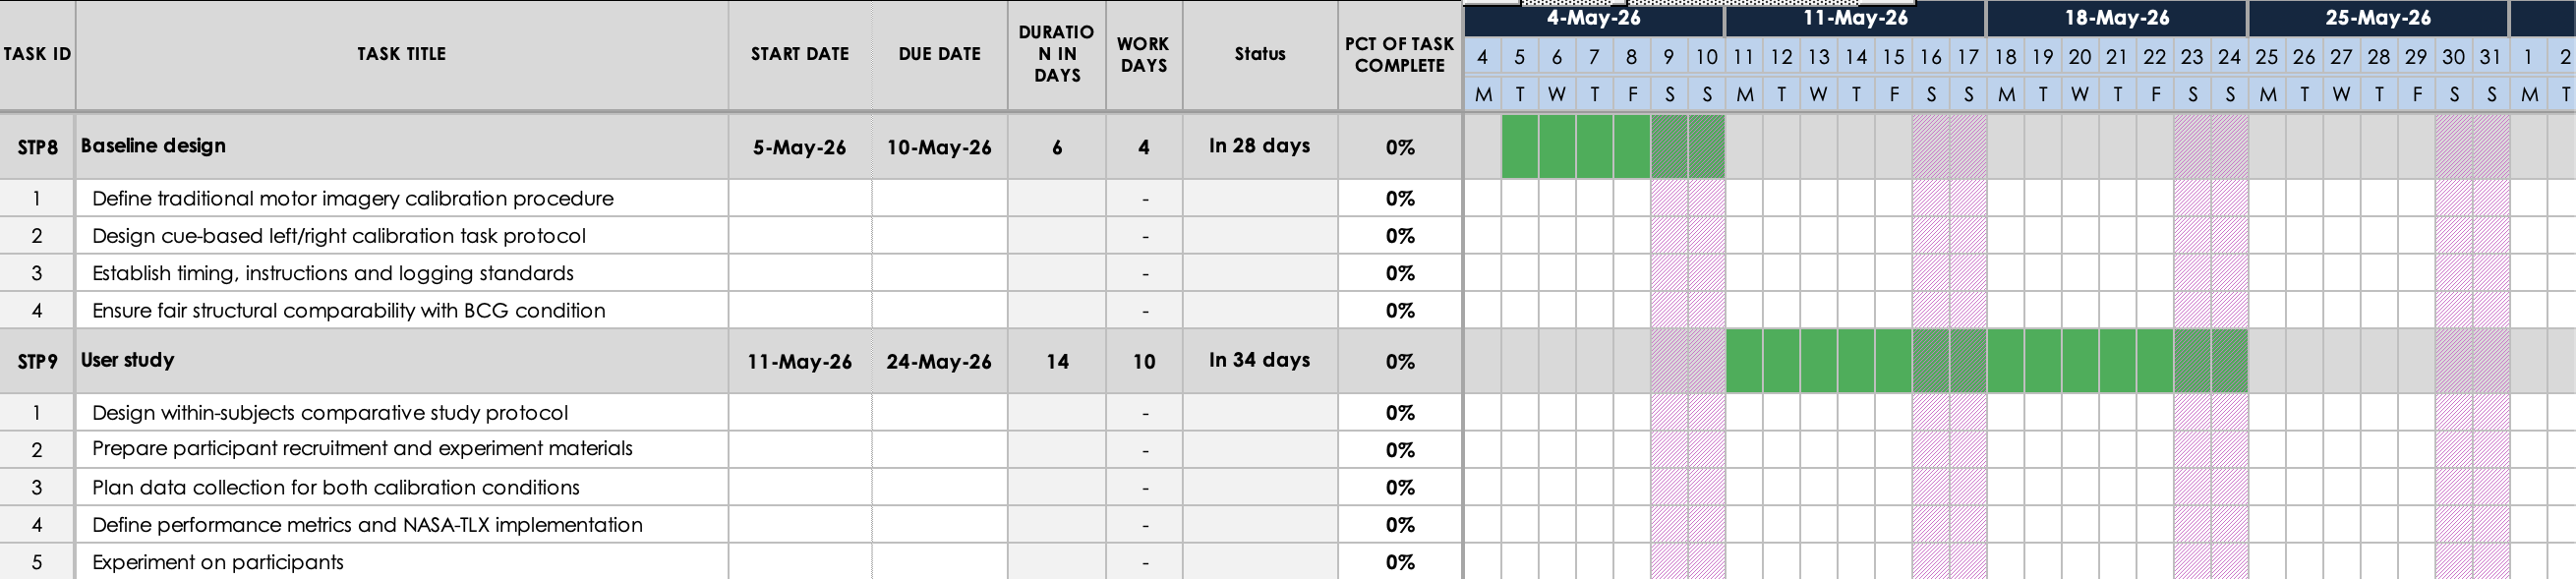
\includegraphics[width=1\textwidth]{Images/timeline-2.png}
        \caption{Project Timeline - May}
        \label{fig:timeline-2}
    \end{figure}

    \newpage
    \begin{figure}[H]
        \centering
        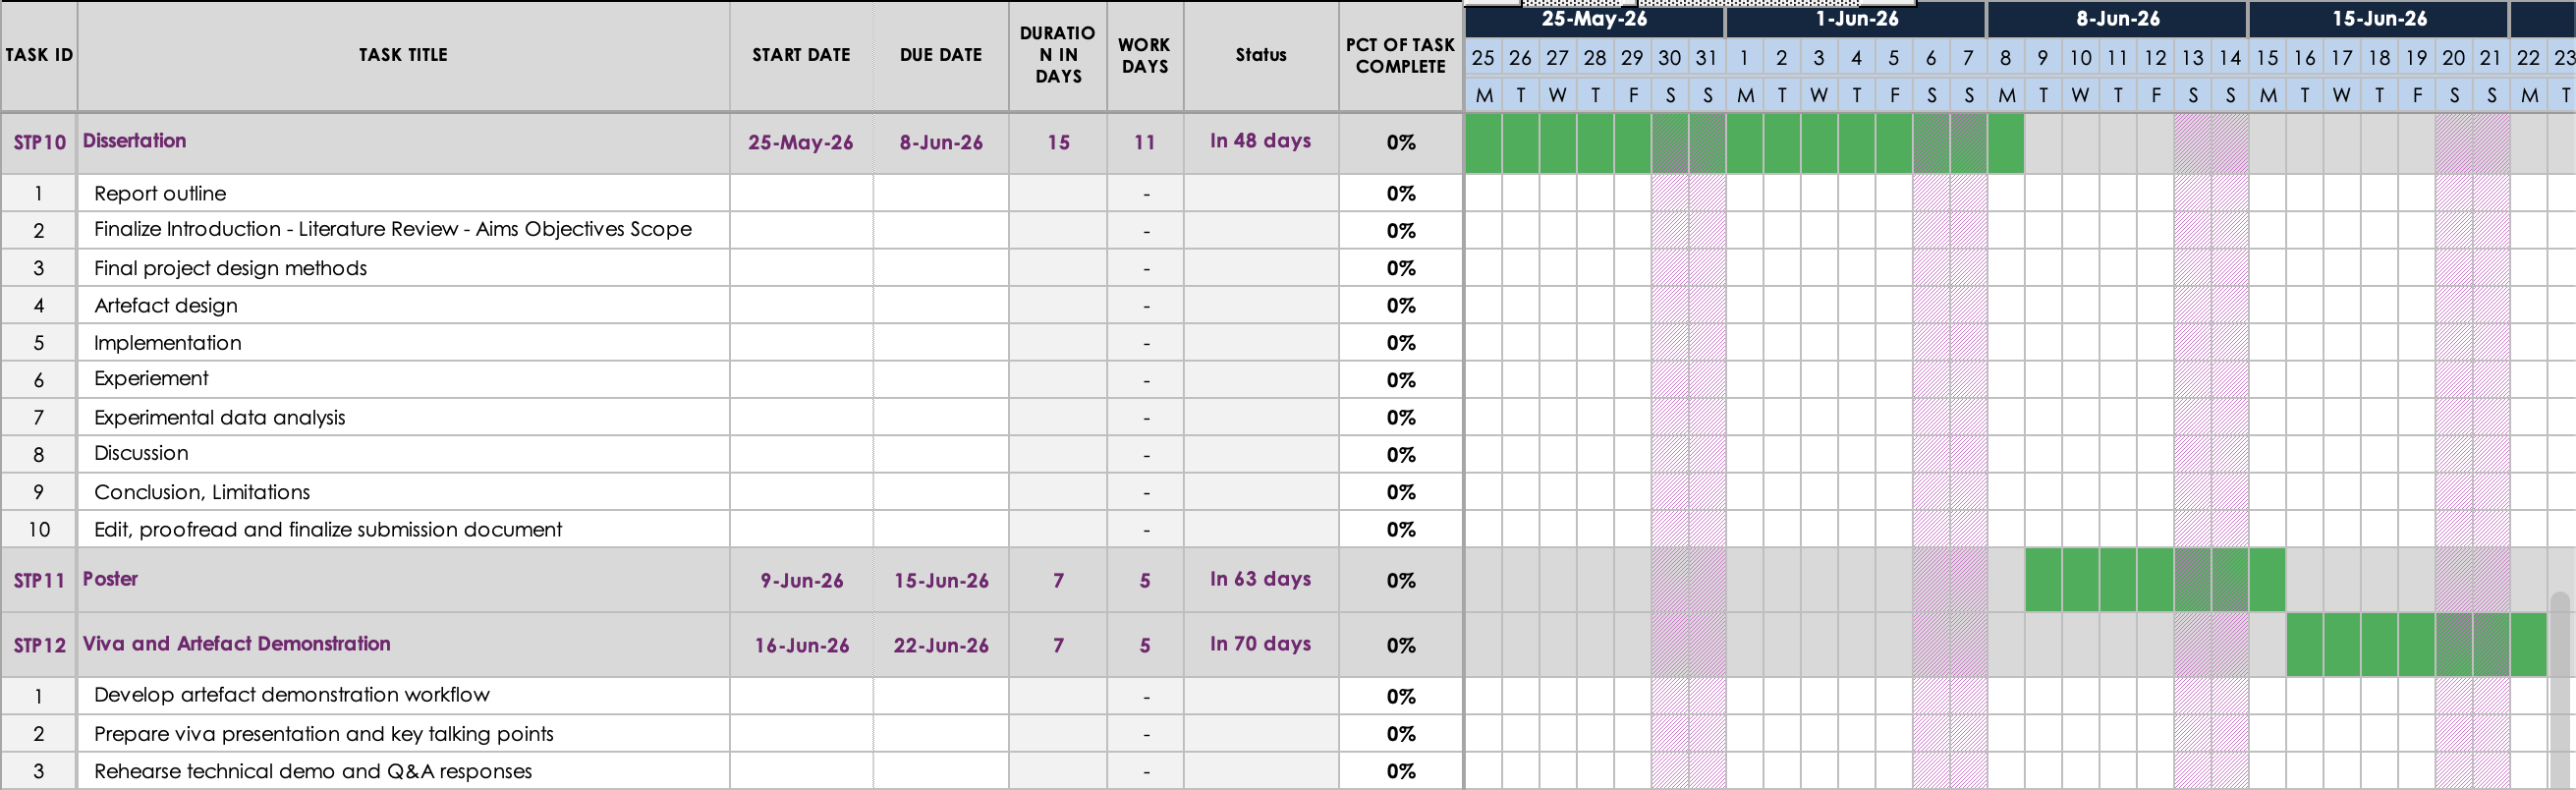
\includegraphics[width=1\textwidth]{Images/timeline-3.png}
        \caption{Project Timeline - June}
        \label{fig:timeline-3}
    \end{figure}


    \section{Draft Outline of Final Report}
    \begin{enumerate}
        \item Introduction
        \item Review of Existing Knowledge
        \item System Requirements and Architecture
        \item EEG Hardware Investigation and Device Selection
        \item Signal Processing and Classification Pipeline
        \item BCG Game Design and Implementation
        \item Real-Time System Integration
        \item Baseline Protocol Design
        \item User Study and Evaluation
        \item Discussion
        \item Conclusion and Future Work
    \end{enumerate}

\end{document}
